%-------------------------
% Resume in Latex
% Author : Zakaria TOZY
%------------------------

\documentclass[11pt,a4paper]{article}

\usepackage{latexsym}
\usepackage[empty]{fullpage}
\usepackage{titlesec}
\usepackage{marvosym}
\usepackage[usenames,dvipsnames]{color}
\usepackage{verbatim}
\usepackage{enumitem}
\usepackage[hidelinks]{hyperref}
\usepackage{fancyhdr}
\usepackage[english,french]{babel}
\usepackage{tabularx}
\usepackage[utf8]{inputenc}
\usepackage[left=0.6in, right=0.6in, top=0.4in, bottom=0.3in]{geometry}

\usepackage{fontawesome}
\usepackage[scale=0.90,lf]{FiraMono}

\definecolor{light-grey}{gray}{0.83}
\definecolor{dark-grey}{gray}{0.3}
\definecolor{text-grey}{gray}{.08}

\DeclareRobustCommand{\ebseries}{\fontseries{eb}\selectfont}
\DeclareTextFontCommand{\texteb}{\ebseries}

\usepackage{contour}
\usepackage[normalem]{ulem}
\renewcommand{\ULdepth}{1.8pt}
\contourlength{0.8pt}
\newcommand{\myuline}[1]{%
  \uline{\phantom{#1}}%
  \llap{\contour{white}{#1}}%
}

\usepackage{tgheros}
\renewcommand*\familydefault{\sfdefault} 
\usepackage[T1]{fontenc}

\usepackage{graphicx}

\pagestyle{fancy}
\fancyhf{} 
\fancyfoot{}
\renewcommand{\headrulewidth}{0pt}
\renewcommand{\footrulewidth}{0pt}

\urlstyle{same}

\raggedbottom
\raggedright
\setlength{\tabcolsep}{0in}

\titleformat{\section}{
    \bfseries \vspace{-4pt} \raggedright \normalsize
}{}{0em}{}[\color{light-grey} {\titlerule[1pt]} \vspace{-2pt}]

\newcommand{\resumeItem}[1]{
  \item\footnotesize{
    {#1 \vspace{-1pt}}
  }
}

\newcommand{\resumeSubheading}[4]{
  \vspace{2pt}\item
    \begin{tabular*}{\textwidth}[t]{l@{\extracolsep{\fill}}r}
      {\small\textbf{#1}} & {\footnotesize#2} \\
      {\footnotesize\textit{#3}} & {\footnotesize\textit{#4}} \\
    \end{tabular*}\vspace{-4pt}
}

\newcommand{\resumeProjectHeading}[2]{
  \item
  {\small#1} \hfill {#2}
}

\newcommand{\resumeSubItem}[1]{\resumeItem{#1}\vspace{-4pt}}

\renewcommand\labelitemii{$\vcenter{\hbox{\tiny$\bullet$}}$}

\newcommand{\resumeSubHeadingListStart}{\begin{itemize}[leftmargin=0in, label={}]}
\newcommand{\resumeSubHeadingListEnd}{\end{itemize}}
\newcommand{\resumeItemListStart}{\begin{itemize}[label={\textbullet}]}
\newcommand{\resumeItemListEnd}{\end{itemize}\vspace{0pt}}

\color{text-grey}

\begin{document}

\begin{center}
  \begin{minipage}[c]{0.2\textwidth}
    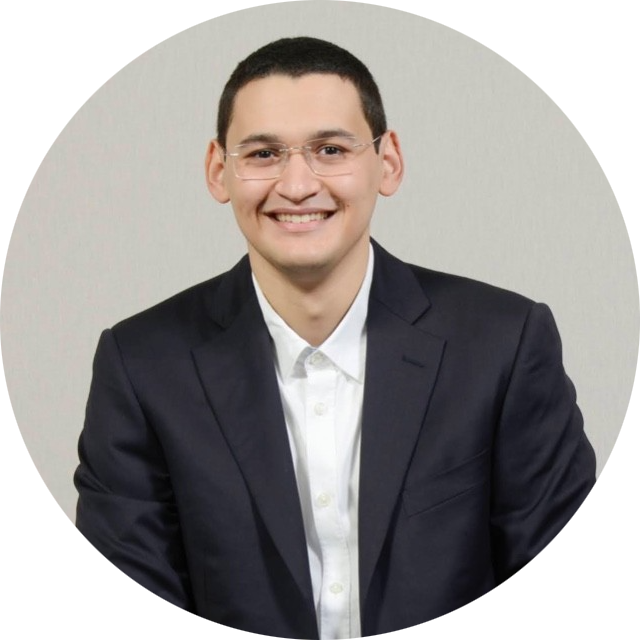
\includegraphics[width=2.5cm]{images/profilpicture.png}
  \end{minipage}%
  \begin{minipage}[c]{0.8\textwidth}
    {\LARGE \textbf{Zakaria TOZY}} \\ \vspace{8pt}
    {\small Data Engineer $|$ CDI} \vspace{5pt}
  \end{minipage}
\end{center}

\vspace{10pt}

\begin{center}
    \small \faPhone\ \texttt{0617407077} \hspace{1pt} $|$
    \hspace{1pt} \faEnvelope\ \texttt{zakaria.tozy@icloud.com} \hspace{1pt} $|$
    \hspace{1pt} \faLinkedin\ \texttt{zakaria-tozy} \hspace{1pt} $|$
    \hspace{1pt} \texttt{CDI} \hspace{1pt} $|$
    \hspace{1pt} \faMapMarker\ \texttt{Paris} \hspace{1pt} $|$
    \hspace{1pt} \faGithub\ \texttt{github.com/zack242} \\ \vspace{10pt}
\end{center}

\begin{itemize}[leftmargin=0in, label={}]
\footnotesize{\item{
Ingénieur en Systèmes d'Information et Data Science avec une double formation (ECE Paris/Polytechnique), passionné par les données et les nouvelles technologies. Je recherche un poste en CDI pour contribuer à des projets innovants et à forte valeur ajoutée.
}}
\end{itemize}

\section{COMPETENCES}
\begin{itemize}[leftmargin=0in, label={}]
\footnotesize{\item{
{\small\textbf{Programming}:} Python, SQL, Java, C++, C{\#} \\
\vspace{3pt}
{\small\textbf{Languages}:} Français (Bilingue), Arabe (Bilingue), Anglais (Courant - TOEIC 875) \\
\vspace{3pt}
{\small\textbf{Machine Learning}:} Scikit-Learn, NLP, Computer Vision, Deep Learning \\
\vspace{3pt}
{\small\textbf{Devops}:} Docker, CI/CD, Git, Scrum \\
\vspace{3pt}
{\small\textbf{Soft Skills}:} Autonomie, Rigueur, Esprit d'analyse, Apprentissage rapide \\
\vspace{3pt}
{\small\textbf{Data & Cloud Engineering}:} PySpark, BigQuery, ETL, Data Pipelines, Databricks, Snowflake, GCP, dbt
}
}
\end{itemize}

\section{EDUCATION}
\resumeSubHeadingListStart
    \resumeSubheading
      {École Centrale d'Électronique (ECE Paris)}
      {Janv 2024}
      {Ingénieur en Systèmes d'Information et Big Data Analytics}
      {Top 5\% de la promotion}
      \resumeItemListStart
        \resumeItem{Spécialisation : Programmation, Bases de données, Électronique, DevOps}
      \resumeItemListEnd
    \resumeSubheading
      {Institut Polytechnique de Paris (Ecole polytechnique)}
      {Janv 2024}
      {Master 2 en Data Sciences}
      {Mention Très bien}
      \resumeItemListStart
        \resumeItem{Spécialisation : Machine Learning, Big Data, Cloud Infrastructure, Deep Learning, NLP}
      \resumeItemListEnd
  \resumeSubHeadingListEnd

\section{EXPERIENCE}
\resumeSubHeadingListStart
    \resumeSubheading
      {AXA Investment Managers - AXA IM}{Août 2023 --- Jan 2024}
      {Data Engineer/Data Analyst Intern}{Paris}
      \resumeItemListStart
        \resumeItem{Conception et mise en place d'une dizaine de pipelines de données pour l'ingestion de données métiers.}
        \resumeItem{Optimisation du modèle de données et migration des pipelines de distribution utilisés pour le reporting financier de 844 milliards d'euros d'actifs en 2023.}
        \resumeItem{Tests de nouveaux clusters sur Databricks et création d'un PoC (Proof of Concept) pour l'anonymisation des données sensibles.}
        \resumeItem{Création de tableaux de bord pour les contrôleurs financiers.}
        \resumeItem{Calcul des indicateurs de performance KPIs pour la vision distribuée (ME, OV, CIS, FX).}
        \resumeItem{Travail sur la qualité et la validation des données d'un ensemble de reporting.}
      \resumeItemListEnd
    \resumeSubheading
      {Kalima Blockchain et IoT}{Avr 2022 --- Août 2022}
      {Software Engineer Intern}{Paris}
      \resumeItemListStart
        \resumeItem{Développement d'un explorateur de blockchain en Java/LevelDB (+1000 transactions par seconde).}
        \resumeItem{Implémentation de nouvelles fonctionnalités d'administration pour la blockchain Kalima en Node.js.}
        \resumeItem{Conception et développement d'un système d'authentification multisignature pour les DApps (Decentralized Applications).}
      \resumeItemListEnd
    \resumeSubheading
      {Le Crédit Lyonnais - LCL}{Janv 2020 --- Fév 2020}
      {IT Intern}{Paris}
      \resumeItemListStart
        \resumeItem{Étude de migration Microsoft Office 2010 vers 2016 et analyse de son impact sur les processus métiers.}
        \resumeItem{Développement et exécution de procédures de tests sur un parc de 23 000 postes de travail.}
      \resumeItemListEnd
  \resumeSubHeadingListEnd

\section{PROJETS}
\resumeSubHeadingListStart
    \resumeProjectHeading
      {\textbf{Bitcoin Analysis}} {}
      \resumeItemListStart
        \resumeItem{Création d'un pipeline de données avec Python, SQL, Airflow, dbt et Snowflake pour l'analyse des transactions Bitcoin, traitant plus de 1 million de transactions par jour.}
      \resumeItemListEnd
    \resumeProjectHeading
      {\textbf{Twitter Real-time Analysis}} {}
      \resumeItemListStart
        \resumeItem{Développement d'un système de visualisation en temps réel des flux Twitter par topics à l'aide de Kafka et de l'algorithme KNN (K-Nearest Neighbors).}
      \resumeItemListEnd
    \resumeProjectHeading
      {\textbf{Energy Disaggregation \@ Capgemini}} {}
      \resumeItemListStart
        \resumeItem{Extraction de la composante thermosensible de la consommation énergétique pour prévoir la demande future en France.}
      \resumeItemListEnd
\resumeSubHeadingListEnd


\end{document} 